%%%%%%%%%%%%%%%%%%%%%%%%%%%%%%%%%%%%%%%%%%%%%%%%%%%%%%%%%%%%%%%%%%%%%%%%%%%%%%%%%%%%%%%%%
% This is a LaTeX template for Bachelor or Master theses at ZHAW, in accordance with the 
% guidelines provided here:
% https://www.zhaw.ch/en/lsfm/study/studiweb/master-ls/masters-thesis/
%
%
% This template is based on previous works by:
% Steve Gunn (http://users.ecs.soton.ac.uk/srg/softwaretools/document/templates/)
% Sunil Patel (http://www.sunilpatel.co.uk/thesis-template/)
% Matteo Delucchi (https://github.com/matteodelucchi/ZHAW_thesis-template)
%
% University specific changes were made by:
% Matteo Delucchi
% Norman Juchler
% 
% Template license:
% CC BY-NC-SA 3.0 (http://creativecommons.org/licenses/by-nc-sa/3.0/)
%%%%%%%%%%%%%%%%%%%%%%%%%%%%%%%%%%%%%%%%%%%%%%%%%%%%%%%%%%%%%%%%%%%%%%%%%%%%%%%%%%%%%%%%%

%----------------------------------------------------------------------------------------
% DOCUMENT SPECIFICATION
%----------------------------------------------------------------------------------------
\documentclass[
    11pt,                      % Default font size
    oneside,                  % One-side binding. Default: Two-side binding / alternating margins
    ngerman,                   % Language. Use ngerman for German (Neue Rechtschreibung)
    singlespacing,             % Spacing option: singlespacing, onehalfspacing or doublespacing
    %nolistspacing,            % Set spacing in lists to single
    %draft,                    % Enable draft mode: no pictures, no links, overfull hboxes indicated
    liststotoc,               % Include list of figures/tables/etc in the table of contents
    toctotoc,                 % Include the main table of contents to the table of contents
    parskip,                  % Add vertical space between paragraphs
    %nohyperref,               % Disable links in the entire document
    helveticafont,             % Uncomment to use Helvetica font
    headsepline,               % Show a horizontal line under the header
    chapterinoneline,         % Place the chapter title and chapter number on one line
    consistentlayout,          % Have the same layout for special chapters: 
                               % declaration, abstract and acknowledgements
]{MastersDoctoralThesis}

% Uncomment the following lines to only include a subset of chapters.
% This is useful for long documents, as typesetting takes a bit of time
%\includeonly{
%    Front/titlepage,
%    Front/imprint,
%    Front/abstract,
%    %Front/declaration,
%    %Front/acknowledgements,
%    %Front/symbols,
%    Chapters/Chapter1,
%    %Chapters/Chapter2
%    }


%----------------------------------------------------------------------------------------
% PREAMBLE: PACKAGES AND CONFIGURATIONS
%----------------------------------------------------------------------------------------
% !TEX root = main.tex
%
% TODO: Have a clearer separation between ZHAW Thesis class and this preamble.

%%%%%%%%%%%%%%%%%%%%%%%%%%%%%%%%%%%%%%%%%%%%%%%%%%%%%%%%%%%%%%%%%%%%%%%%%%%%%%%%
% Fonts and characters
%%%%%%%%%%%%%%%%%%%%%%%%%%%%%%%%%%%%%%%%%%%%%%%%%%%%%%%%%%%%%%%%%%%%%%%%%%%%%%%%

% Support for special characters
\usepackage[utf8]{inputenc}    % Input encoding: Support non-ascii characters
\usepackage[T1]{fontenc}       % Font encoding: T1 is good choice for Europe

% Set main fonts
% Fonts catalogue: https://tug.org/FontCatalogue/
\usepackage{mathpazo}          % Use the Palatino font by default
\usepackage{beramono}          % Override the monospace/typewriter font

\usepackage{amssymb}           % Maths
\usepackage{amsmath}           % Maths 
\usepackage{numprint}          % For nicely printing large numbers
\usepackage{lmodern}           % Use LaTeX math fonts, requires T1


% ZHAW title font
% Try to load Helvetica Rounded Bold, and OpenType font.
% Loading OTF or system fonts is possible with XeLaTeX.
% If the document is compiled using pdfLaTeX, resort 
\usepackage{ifxetex}
\ifxetex
    \usepackage{fontspec}
    \newfontfamily\zhawtitlefont{Helvetica Rounded Bold}
\else
    \newcommand{\zhawtitlefont}{\scshape}
\fi

\newcommand{\boldit}[1]{\textit{\textbf{#1}}}

% Set Helvetica as the default font
\usepackage[scaled]{helvet}
\renewcommand{\familydefault}{\sfdefault}

%%%%%%%%%%%%%%%%%%%%%%%%%%%%%%%%%%%%%%%%%%%%%%%%%%%%%%%%%%%%%%%%%%%%%%%%%%%%%%%%
% Colors
%%%%%%%%%%%%%%%%%%%%%%%%%%%%%%%%%%%%%%%%%%%%%%%%%%%%%%%%%%%%%%%%%%%%%%%%%%%%%%%%

% Set up colors
\usepackage[dvipsnames]{xcolor} % Color management
% ZHAW Blue: Pantone 2945 U / R0 G100 B166
\definecolor{zhawblue}{rgb}{0.00, 0.39, 0.65}
\definecolor{zhawlightblue}{rgb}{0.82, 0.88, 0.93}
% Colors related to code listings
\definecolor{codegreen}{rgb}{0,0.6,0}
\definecolor{codegray}{rgb}{0.5,0.5,0.5}
\definecolor{codepurple}{rgb}{0.58,0,0.82}
\definecolor{codebackground}{rgb}{0.93,0.94,0.95}
% Colors related to tables
\definecolor{tablegray}{rgb}{0.9,0.9,0.9}
\colorlet{tableheader}{tablegray}
% Colors related to hyperref
\definecolor{linkcolor}{rgb}{0.1, 0.1, 0.1}

%%%%%%%%%%%%%%%%%%%%%%%%%%%%%%%%%%%%%%%%%%%%%%%%%%%%%%%%%%%%%%%%%%%%%%%%%%%%%%%%
% Environments
%%%%%%%%%%%%%%%%%%%%%%%%%%%%%%%%%%%%%%%%%%%%%%%%%%%%%%%%%%%%%%%%%%%%%%%%%%%%%%%%

\usepackage[ngerman]{babel}    % Language support

\usepackage[                    % Create hypertext links
    colorlinks=true, 
    allbordercolors={white}, 
    linkcolor=linkcolor, 
    citecolor=linkcolor, 
    filecolor=linkcolor, 
    urlcolor=linkcolor]{hyperref}

\usepackage{graphicx}          % Include graphics
\usepackage{tabularx}          % Create nicer tables
\usepackage{booktabs}          % To further beautify tables

\usepackage{caption}           % Customized caption
\usepackage{subcaption}        % Subfigure captions
\usepackage{makecell}          % Per-cell formatting in tables (\makecell)
\usepackage{pdfpages}          % Required to include PDF files/graphics (\includepdf)
\usepackage{colortbl}          % Tables with colors

\usepackage{todonotes}         % Introduces the command \todo
\setlength{\marginparwidth}{2.5cm} % Adjust this if the todo notes are out of margins
\usepackage{array,ragged2e}    % For ragged alignment of multi-line table cells

% Adjust tables
\colorlet{tableheadcolor}{gray!25}                % Table header colour
\newcommand{\headcol}{\rowcolor{tableheadcolor}}% % The color of the head
\newcommand{\topline}{\arrayrulecolor{black}      %
                      \specialrule{0.1em}{\abovetopsep}{0.5pt}%
                      \arrayrulecolor{tableheadcolor}%
                      \specialrule{\belowrulesep}{0pt}{-3pt}%
            \arrayrulecolor{black}
            }
\newcommand{\midline}{\arrayrulecolor{tableheadcolor}
            \specialrule{\aboverulesep}{-1pt}{0pt}%
            \arrayrulecolor{black}\specialrule{\lightrulewidth}{0pt}{0pt}%
            \arrayrulecolor{white}\specialrule{\belowrulesep}{0pt}{-3pt}%
            \arrayrulecolor{black}
            }
\newcommand{\bottomline}{\arrayrulecolor{white}\specialrule{\aboverulesep}{0pt}{-2pt}%
            \arrayrulecolor{black}\specialrule{\heavyrulewidth}{0pt}{\belowbottomsep}}%

% Create boxes as follows:
% \begin{colorbox}{red}{2}
\usepackage{tcolorbox}
\newtcolorbox{textbox}[2]{
    arc=3pt,
    boxrule=#2pt,
    colback=#1!25!white,
    width=\textwidth,
    halign=left,
    valign=center,
    colframe=#1!75!black
}

%%%%%%%%%%%%%%%%%%%%%%%%%%%%%%%%%%%%%%%%%%%%%%%%%%%%%%%%%%%%%%%%%%%%%%%%%%%%%%%%
% Code listings
%%%%%%%%%%%%%%%%%%%%%%%%%%%%%%%%%%%%%%%%%%%%%%%%%%%%%%%%%%%%%%%%%%%%%%%%%%%%%%%%
\captionsetup{format=plain,             % plain or hang
              justification=justified,  % justified, centering, raggedright, ...
              labelfont=bf,
              font=small,
              margin=20pt}
              

%%%%%%%%%%%%%%%%%%%%%%%%%%%%%%%%%%%%%%%%%%%%%%%%%%%%%%%%%%%%%%%%%%%%%%%%%%%%%%%%
% Code listings
%%%%%%%%%%%%%%%%%%%%%%%%%%%%%%%%%%%%%%%%%%%%%%%%%%%%%%%%%%%%%%%%%%%%%%%%%%%%%%%%

\newcommand{\code}[1]{\texttt{#1}}

% Setup code listings
\usepackage{listings}
\lstdefinestyle{mystyle}{
    backgroundcolor=\color{codebackground},   
    commentstyle=\color{codegreen},
    keywordstyle=\color{magenta},
    numberstyle=\tiny\color{codegray},
    stringstyle=\color{codepurple},
    basicstyle=\ttfamily\scriptsize,
    breakatwhitespace=false,
    breaklines=true,
%    captionpos=b,
    keepspaces=true,
    numbers=left,
    numbersep=5pt,
    showspaces=false,
    showstringspaces=false,
    showtabs=false,
    tabsize=4
}
\lstset{style=mystyle}

% minted is an alternative code listing package. (See appendix A)
% For it to run successfully, ensure the following:
% - the Python package Pygments. Install with the following command:
%       python -m pip install Pygments
% - pdflatex (or xelatex) is executed with the flag --shell-escape
%   If you are using a TEX editor, you can modify the typesetting 
%   command somewhere in the settings.
%\usepackage[outputdir=build]{minted}
%\usemintedstyle{xcode}
% For fancier coloring schemes, see here:
% https://tex.stackexchange.com/questions/585582
% One could also create an own style in Pygments
% https://pygments.org/docs/styles/#creating-own-styles


%%%%%%%%%%%%%%%%%%%%%%%%%%%%%%%%%%%%%%%%%%%%%%%%%%%%%%%%%%%%%%%%%%%%%%%%%%%%%%%%
% References
%%%%%%%%%%%%%%%%%%%%%%%%%%%%%%%%%%%%%%%%%%%%%%%%%%%%%%%%%%%%%%%%%%%%%%%%%%%%%%%%

% Set up references
\usepackage[
    backend=biber,             % Use biber backend (an external tool)
    sorting=none,              % Enumerates the reference in order of their appearance
    style=authoryear           % Choose here your preferred citation style
]{biblatex}
\addbibresource{SA1.bib} % The filename of the bibliography
\usepackage[autostyle=true]{csquotes} 
                               % Required to generate language-dependent quotes 
                               % in the bibliography


%%%%%%%%%%%%%%%%%%%%%%%%%%%%%%%%%%%%%%%%%%%%%%%%%%%%%%%%%%%%%%%%%%%%%%%%%%%%%%%%
% MARGIN SETTINGS
%%%%%%%%%%%%%%%%%%%%%%%%%%%%%%%%%%%%%%%%%%%%%%%%%%%%%%%%%%%%%%%%%%%%%%%%%%%%%%%%
\usepackage{geometry}
\geometry{
    paper=a4paper,       % Change to letterpaper for US letter
    %inner=2.5cm,        % Inner margin
    %outer=3.8cm,        % Outer margin
    %top=1.5cm,          % Top margin
    bottom=4.cm,         % Bottom margin
    bindingoffset=.5cm,  % Binding offset
    %showframe,          % Show the type block of the page
}

% Other layout settings
\setlength\parindent{0em} % No indent
\setlength{\parskip}{1em}
%\usepackage{parskip}


\setlength{\intextsep}{30pt}   % Distance between image and text 
\usepackage{enumitem}          % Layout control for list environments (e.g, itemize)
\setlist{noitemsep}            % Suppress extra spaces between items
%\setlist{nosep}               % Suppress spaces before/after list environments


%----------------------------------------------------------------------------------------
%   PENALTIES
%----------------------------------------------------------------------------------------

\doublehyphendemerits=10000 % No consecutive line hyphens
\brokenpenalty=10000 % No broken words across columns/pages
\widowpenalty=9999 % Almost no widows at bottom of page
\clubpenalty=9999 % Almost no orphans at top of page
\interfootnotelinepenalty=9999 % Almost never break footnotes


%%%%%%%%%%%%%%%%%%%%%%%%%%%%%%%%%%%%%%%%%%%%%%%%%%%%%%%%%%%%%%%%%%%%%%%%%%%%%%%%
% MANAGE AUTHOR LISTS
%%%%%%%%%%%%%%%%%%%%%%%%%%%%%%%%%%%%%%%%%%%%%%%%%%%%%%%%%%%%%%%%%%%%%%%%%%%%%%%%

\usepackage[affilmode=count]{authors}


% Trick: Convert the setter into a getter.
\NewDocumentCommand{\projecttitle}{m}{\renewcommand{\projecttitle}{#1}}
\NewDocumentCommand{\projecttype}{m}{\renewcommand{\projecttype}{#1}}
\NewDocumentCommand{\projectcode}{m}{\renewcommand{\projectcode}{#1}}
\NewDocumentCommand{\projectdate}{m}{\renewcommand{\projectdate}{#1}}
\NewDocumentCommand{\keywords}{m}{\renewcommand{\keywords}{#1}}

\NewDocumentCommand{\university}{m}{\renewcommand{\university}{#1}}
\NewDocumentCommand{\department}{m}{\renewcommand{\department}{#1}}
\NewDocumentCommand{\institute}{m}{\renewcommand{\institute}{#1}}
\NewDocumentCommand{\group}{m}{\renewcommand{\group}{#1}}


%----------------------------------------------------------------------------------------
%   HEADERS AND FOOTERS
%----------------------------------------------------------------------------------------

% Notes:
% - In twoside mode, left and right side pages may differ
% - Pages: left = even, right = odd
%   Chapters usually are forced to start at odd pages.
% - \markboth{left}{right} how left and right pages are marked
% - \automark is a convenience command from the scrlayer-scrpage package. It issues 
%   that \markboth is called for every \chapter and \section command.
% - Historical note: scrlayer-scrpage is the successor of scrpage2
% - Refs:
%    \markboth:  https://tex.stackexchange.com/questions/198676
%    \automark:  https://tex.stackexchange.com/questions/34269/
%    \automark*: https://tex.stackexchange.com/questions/348550/
%
\usepackage[markcase=used]{scrlayer-scrpage}
\ifoot{}% Empty inner footer by default
\ofoot{}% Empty outer footer by default
\providepairofpagestyles{basicStyle}{
    % Header specs for style basicStyle
    \clearpairofpagestyles%
    % \automark[section]{section}
    % \ihead{\headmark}% Inner header
    % \ohead[\pagemark]{\pagemark}% Outer header
    \cfoot[\pagemark]{\pagemark}% Footer with pagemark in the middle
}
\pagestyle{basicStyle}

\providepairofpagestyles[basicStyle]{reportStyle}{%
    \automark*[subsection]{}% Override right marks with section title once one is set
                         % Otherwise, use the chapter title -> basicStyle
}
% \pagestyle{reportStyle}

\KOMAoption{headsepline}{false} % set true to get a line below the header









%----------------------------------------------------------------------------------------
% THESIS INFORMATION: MODIFY THIS SECTION!
%----------------------------------------------------------------------------------------

% The information below is used in the following parts:
% - Title page
% - Imprint
% - Abstract / Zusammenfassung
% - Meta information of PDF

\thesistitle{Titration von Aminosäuren}             % Thesis title,              command: \ttitle
\thesistype{Laborbericht}             % Type of thesis (e.g. Master Thesis) \ttype
\thesisdate{\today}                     % Date of submission                  \tdate
\keywords{gravity, physics, disruptive science}
                                        % Keywords for the thesis,            \keywordnames
\author{Jonas Iseli\\ Julian Kraft}                  % Your name,                          \authorname
\degree{Bachelor of Science}          % Degree name,                        \degreename
\studyprogram{Umweltingenieurswesen} 
                                        % Study program                       \studyprog
\studyprogramlink{https://www.zhaw.ch/en/lsfm/study/master/applied-computational-life-sciences/}
                                        % Link to study program               \studyproglink

\supervisorA{Fabio Rezzonico}       % Name of supervisor 1,               \supnameA
\supervisorAmail{e=mc2@zhaw.ch}         % Email address of supervisor 1,      \supmailA
\supervisorAweb{https://en.wikipedia.org/wiki/Albert\_Einstein}  %            \supwebA
\supervisorAinfo{                       % Formatted info about supervisor 1:  \supinfoA
    \supnameA\\
    Zurich University of Applied Sciences\\
    Email: \href{mailto:\supmailA}{\supmailA}\\
    Web: \href{\supwebA}{Link}
}

% Keep empty if there is no supervisor 2: \supervisorB{}
\supervisorB{Lukas Muri}              % Name of supervisor 2,               \supnameB
\supervisorBmail{f=am@newton.com}       % Email address of supervisor 2,      \supmailB
\supervisorBweb{https://en.wikipedia.org/wiki/John\_Locke}                  % \supwebB
\supervisorBinfo{                       % Formatted info about supervisor 2:  \supinfoB
    \supnameB\\
    University of Cambridge\\
    Email: \href{mailto:\supmailB}{\supmailB}\\
    Web: \href{\supwebB}{Link}
}

\university{Zurich University of Applied Sciences}
                                        % University name                     \univname
\universitygerman{Zürcher Hochschule für Angewandte Wissenschaften}
                                        % University, in German               \univnameger
\department{Life Sciences und Facility Management} 
                                        % Department,                         \deptname
\institute{Institut für Umwelt und Natürliche Resourcen} 
                                        % Institute,                          \instname
\group{Center of Computational Health} 
                                        % Research group                      \groupname

% Links
\universitylink      {https://www.zhaw.ch/en/university/}                   % \univlink
\universitylinkgerman{https://www.zhaw.ch/de/university/}                   % \univlinkger
\departmentlink      {https://www.zhaw.ch/de/lsfm/}                         % \deptlink
\institutelink       {https://www.zhaw.ch/en/lsfm/institutes-centres/icls/} % \instlink
\grouplink           {https://www.zhaw.ch/en/lsfm/institutes-centres/icls/computational-health/} % \grplink



\AtBeginDocument{
\hypersetup{pdftitle=\ttitle} % Set the PDF's title to your title
\hypersetup{pdfauthor=\authorname} % Set the PDF's author to your name
\hypersetup{pdfkeywords=\keywordnames} % Set the PDF's keywords to your keywords
}

\begin{document}
\frontmatter                  % Roman page numbering for the pre-content pages
\pagestyle{plain}             % Default to the plain heading style until the thesis style 
                              % is called for the body content


%----------------------------------------------------------------------------------------
% TITLE PAGE AND IMPRINT
%----------------------------------------------------------------------------------------
% !TEX root = ../main.tex

%%%%%%%%%%%%%%%%%%%%%%%%%%%%%%%%%%%%%%%%%%%%%%%%%%%%%%%%%%%%%%%%%%%%%%%%%%%%%%%%
% TITLE PAGE
%%%%%%%%%%%%%%%%%%%%%%%%%%%%%%%%%%%%%%%%%%%%%%%%%%%%%%%%%%%%%%%%%%%%%%%%%%%%%%%%

% New command to make the lines in the title page
\newcommand{\HRule}{\rule{.9\linewidth}{.6pt}} 

\newgeometry{margin=1in}
\begin{titlepage}

% Make the title page mostly inert to the parskip-setting.
\setlength{\parskip}{0pt}

\begin{center}

\includegraphics[width=0.15\textwidth]{Figures/zhaw_rgb}

\ifxetex
    \vspace{0.6cm}
    {\zhawtitlefont\color{zhawblue}\LARGE\university\par}   % University
    \vspace{0.2cm}
\else
    \vspace{0.87cm}
    {
\includegraphics[height=17.9pt]{figures/zhaw_font_eng_font}\par}
    \vspace{0.05cm}
\fi
{\Large \ifdefempty{\department}{}{Department \department\par}} % Department
\vspace{0.2cm}
{\Large \institute\par}                                     % Institute
\vspace{3.5cm}                            
\textsc{\Large \projecttype}                                % Project type
\vspace{0.2cm}
\HRule 
\vspace{0.4cm}
{\huge \bfseries \projecttitle\par}                         % Project title
\vspace{0.4cm}  
\HRule
\vspace{1.5cm}



\begin{footnotesize}
\begin{tabular}{lr}

% Authors
\begin{minipage}[t]{0.41\textwidth}
\begin{flushleft}
    \boldit{Authors:}\\
    \printauthors[\\][email3]% No whitespace!
    \vspace{1cm}
\end{flushleft}
\end{minipage}

&

% Collaborators
\begin{minipage}[t]{0.41\textwidth}
\begin{flushright}
    \boldit{Collaborators:} \\
    \printcollaborators[\\][email3]% No whitespace!
    \vspace{1cm}
\end{flushright}
\end{minipage}

\\

% Affiliations
\begin{minipage}[t]{0.41\textwidth}
\begin{flushleft}
    \boldit{Affiliations:} \\
    \printaffiliations[\\]
\end{flushleft}
\end{minipage}

&

% Industrial partners
\begin{minipage}[t]{0.41\textwidth}
\begin{flushright}
    \boldit{Industry partner:} \\
    \printcompanies[\\]
\end{flushright}
\end{minipage}

\end{tabular}
\end{footnotesize}

% \begin{footnotesize}
% \begin{minipage}[t]{0.4\textwidth}
% \begin{flushleft}
%     \emph{Authors:}\\
%     \printauthors[\\][compact]\\
%     \vspace{0.5cm}
%     \emph{Affiliations:} \\
%     \printaffiliations[\\]
% \end{flushleft}
% \end{minipage}
% \begin{minipage}[t]{0.4\textwidth}
% \begin{flushright}
%     \emph{Partners:} \\
%     \printcollaborators[\\][compact]\\
%     \vspace{0.5cm}
%     \emph{Industrial partner:} \\
%     \printcompanies[\\]
% \end{flushright}
% \end{minipage}
% \end{footnotesize}

\vspace{2cm}
 
\vfill

{\large
\projectdate\\
\vspace{1.5cm}
Project Code:\\
\projectcode
}
\vfill
\end{center}
\end{titlepage}
\restoregeometry

 \let\cleardoublepage\clearpage
% % !TEX root = ../main.tex

%----------------------------------------------------------------------------------------
% IMPRINT
%----------------------------------------------------------------------------------------

\thispagestyle{empty}
\vspace*{\fill}

\section*{Imprint}
%\vspace{0.75cm}

\begin{footnotesize}


\begin{flushleft} 
\begin{tabular}{ @{}lp{0.6\textwidth}@{} } 
\emph{Project type:}        & \projecttype\\
\emph{Title}:               & \projecttitle\\
\emph{Code}:                & \projectcode\\
\emph{Date}:                & \projectdate\\
\emph{Keywords}:            & \keywords\\
\emph{Copyright}:           & \university\\[0.75cm]
\emph{Authors}:             & \printauthors[\newline][email2]\\
\emph{Collaborators:}       & \printcollaborators[\newline][email2]\\
\emph{Affiliations}:        & \printaffiliations[\newline]\\
                            & \printcompanies[\newline]\\
\end{tabular}
\end{flushleft}


\end{footnotesize}



%----------------------------------------------------------------------------------------
% DECLARATION
%----------------------------------------------------------------------------------------
% Comment out this section if the declaration of originality from ZHAW is used.
% % !TEX root = ../main.tex

%----------------------------------------------------------------------------------------
% DECLARATION OF ORIGINALITY
%----------------------------------------------------------------------------------------

\begin{declaration}
\addchaptertocentry{\authorshipname} % Add the declaration to the table of contents

\begin{textbox}{red}{2}
REMOVE THIS SECTION IF THE \href{https://www.zhaw.ch/en/lsfm/study/studiweb/master-ls/masters-thesis/}{ORIGINAL COPY OF THE ZHAW DECLARATION OF ORIGINALITY} IS USED IN THE APPENDIX.
\end{textbox}
\vspace{1cm}

\noindent I, \authorname, declare that this thesis titled, \enquote{\ttitle} and the work presented in it are my own. I confirm that:

\begin{itemize} 
\item This work was done wholly or mainly while in candidature for a research degree at the \univname.
\item Where any part of this thesis has previously been submitted for a degree or any other qualification at this university or any other institution, this has been clearly stated.
\item Where I have consulted the published work of others, this is always clearly attributed.
\item Where I have quoted from the work of others, the source is always given. With the exception of such quotations, this thesis is entirely my own work.
\item I have acknowledged all main sources of help.
\item Where the thesis is based on work done by myself jointly with others, I have made clear exactly what was done by others and what I have contributed myself.\\
\end{itemize}
\vspace{1cm}

\noindent Signed:\\
\rule[0.5em]{25em}{0.5pt} % This prints a line for the signature
 
\noindent Date:\\
\rule[0.5em]{25em}{0.5pt} % This prints a line to write the date
\end{declaration}

% \cleardoublepage


%----------------------------------------------------------------------------------------
% ABSTRACT
%----------------------------------------------------------------------------------------
% Indicate the main file. Must go at the beginning of the file.
% !TEX root = ../main.tex

%%%%%%%%%%%%%%%%%%%%%%%%%%%%%%%%%%%%%%%%%%%%%%%%%%%%%%%%%%%%%%%%%%%%%%%%%%%%%%%%
% Abstract
%%%%%%%%%%%%%%%%%%%%%%%%%%%%%%%%%%%%%%%%%%%%%%%%%%%%%%%%%%%%%%%%%%%%%%%%%%%%%%%%

\vspace*{\fill}

\section*{Abstract}
\label{abstract}

Biodiversity is rapidly declining worldwide. The first step towards understanding the causes and taking measures to counteract this trend is the development of methods and tools to quantify and monitor it. 
The biodiversity of insects is highly relevant due to their crucial role in ecosystems.
Insects contribute to processes such as pollination, decomposition, and serving as a food source for other species.
While many methods exist to monitor insects, ecoacoustics provides a non-invasive paradigm to measure species via acoustic signals.
Recently, data-driven approaches, particularly deep learning-based methods, have proven effective in detecting insect species from acoustic in situ field measurements.
These advancements offer promising new ways to understand, monitor, and protect insect populations.
This study aims to reproduce the results of a previous research on insect sound 
classification using deep learning and to assess the accessibility of this technology. 
Using the InsectSet32 dataset, which contains 335 recordings of 32 insect species, a 
convolutional neural network (CNN) with residual blocks (ResNet) was developed. 
The model was implemented and trained using the 
PyTorch framework and optimized via hyperparameter tuning. The best-performing model 
achieved an accuracy of 0.706 on the validation set and 0.649 on the test set, 
closely aligning with the original study's findings. This work demonstrates that, 
with appropriate knowledge and relatively affordable hardware, such as a regular 
gaming computer equipped with a graphics processing unit (GPU), non-experts can effectively utilize deep 
learning models for ecoacoustic applications. The study underscores the potential 
of combining ecoacoustics with artificial intelligence to advance biodiversity monitoring, 
providing a non-invasive and efficient method for large-scale environmental assessments.

\vspace*{\fill}


%----------------------------------------------------------------------------------------
% ACKNOWLEDGEMENTS
% %----------------------------------------------------------------------------------------
% % !TEX root = ../main.tex

%----------------------------------------------------------------------------------------
% ACKNOWLEDGEMENTS
%----------------------------------------------------------------------------------------
\begin{acknowledgements}
\addchaptertocentry{\acknowledgementname} % Add the acknowledgements to the table of contents

The acknowledgements belong here. Do not forget to mention your project supervisors, without flattering them too much.
\end{acknowledgements}



%----------------------------------------------------------------------------------------
% LIST OF CONTENTS/FIGURES/TABLES PAGES
%----------------------------------------------------------------------------------------
% Comment out if any of the following is not needed:
\tableofcontents  % Add main table of contents
%\listoffigures    % Add list of figures
%\listoftables     % Add list of tables


%----------------------------------------------------------------------------------------
% ABBREVIATIONS / SYMBOLS
%----------------------------------------------------------------------------------------
% % !TEX root = ../main.tex

%----------------------------------------------------------------------------------------
% ABBREVIATIONS
%----------------------------------------------------------------------------------------

% List of abbreviations: a table of two columns.
\begin{abbreviations}{ll}

\textbf{LAH} & \textbf{L}ist \textbf{A}bbreviations \textbf{H}ere\\
\textbf{WSF} & \textbf{W}hat (it) \textbf{S}tands \textbf{F}or\\

\end{abbreviations}


%----------------------------------------------------------------------------------------
% PHYSICAL CONSTANTS/OTHER DEFINITIONS
%----------------------------------------------------------------------------------------

%% List of physical constants: a three column table
%\begin{constants}{lr@{${}={}$}l} 
%
%% The \SI{}{} command is provided by the siunitx package, see its documentation 
%% for instructions on how to use it
%
%Speed of Light & $c_{0}$ & \SI{2.99792458e8}{\meter\per\second} (exact)\\
%%Constant Name & $Symbol$ & $Constant Value$ with units\\
%
%\end{constants}


%----------------------------------------------------------------------------------------
% SYMBOLS
%----------------------------------------------------------------------------------------

%% List of Symbols: a three column table
%\begin{symbols}{lll} 
%
%$a$ & distance & \si{\meter} \\
%$P$ & power & \si{\watt} (\si{\joule\per\second}) \\
%%Symbol & Name & Unit \\
%
%\addlinespace % Gap to separate the Roman symbols from the Greek
%
%$\omega$ & angular frequency & \si{\radian} \\
%
%\end{symbols}



%----------------------------------------------------------------------------------------
% DEDICATION
%----------------------------------------------------------------------------------------
% \dedicatory{For/Dedicated to/To my\ldots} 


%----------------------------------------------------------------------------------------
% THESIS CONTENT - CHAPTERS
%----------------------------------------------------------------------------------------
\mainmatter % Begin numeric (1,2,3...) page numbering
\pagestyle{thesis} % Return the page headers back to the "thesis" style

% Include the chapters of the thesis as separate files from the Chapters folder
% Uncomment the lines as you write the chapters

% Indicate the main file. Must go at the beginning of the file.
% !TEX root = ../main.tex

%----------------------------------------------------------------------------------------
% CHAPTER TEMPLATE
%----------------------------------------------------------------------------------------


\chapter{Einleitung} % Main chapter title

\label{Chapter1} % Change X to a consecutive number; for referencing this chapter elsewhere, use \ref{ChapterX}

%----------------------------------------------------------------------------------------
% SECTION 1
%----------------------------------------------------------------------------------------

\section{Main Section 1}

Lorem ipsum dolor sit amet, consectetur adipiscing elit. Aliquam ultricies lacinia euismod. Nam tempus risus in dolor rhoncus in interdum enim tincidunt. Donec vel nunc neque. In condimentum ullamcorper quam non consequat. Fusce sagittis tempor feugiat. Fusce magna erat, molestie eu convallis ut, tempus sed arcu. Quisque molestie, ante a tincidunt ullamcorper, sapien enim dignissim lacus, in semper nibh erat lobortis purus. Integer dapibus ligula ac risus convallis pellentesque.

%-----------------------------------
% SUBSECTION 1
%-----------------------------------
\subsection{Subsection 1}

Nunc posuere quam at lectus tristique eu ultrices augue venenatis. Vestibulum ante ipsum primis in faucibus orci luctus et ultrices posuere cubilia Curae; Aliquam erat volutpat. Vivamus sodales tortor eget quam adipiscing in vulputate ante ullamcorper. Sed eros ante, lacinia et sollicitudin et, aliquam sit amet augue. In hac habitasse platea dictumst.

%-----------------------------------
% SUBSECTION 2
%-----------------------------------

\subsection{Subsection 2}
Morbi rutrum odio eget arcu adipiscing sodales. Aenean et purus a est pulvinar pellentesque. Cras in elit neque, quis varius elit. Phasellus fringilla, nibh eu tempus venenatis, dolor elit posuere quam, quis adipiscing urna leo nec orci. Sed nec nulla auctor odio aliquet consequat. Ut nec nulla in ante ullamcorper aliquam at sed dolor. Phasellus fermentum magna in augue gravida cursus. Cras sed pretium lorem. Pellentesque eget ornare odio. Proin accumsan, massa viverra cursus pharetra, ipsum nisi lobortis velit, a malesuada dolor lorem eu neque.

%----------------------------------------------------------------------------------------
% SECTION 2
%----------------------------------------------------------------------------------------

\section{Main Section 2}

Sed ullamcorper quam eu nisl interdum at interdum enim egestas. Aliquam placerat justo sed lectus lobortis ut porta nisl porttitor. Vestibulum mi dolor, lacinia molestie gravida at, tempus vitae ligula. Donec eget quam sapien, in viverra eros. Donec pellentesque justo a massa fringilla non vestibulum metus vestibulum. Vestibulum in orci quis felis tempor lacinia. Vivamus ornare ultrices facilisis. Ut hendrerit volutpat vulputate. Morbi condimentum venenatis augue, id porta ipsum vulputate in. Curabitur luctus tempus justo. Vestibulum risus lectus, adipiscing nec condimentum quis, condimentum nec nisl. Aliquam dictum sagittis velit sed iaculis. Morbi tristique augue sit amet nulla pulvinar id facilisis ligula mollis. Nam elit libero, tincidunt ut aliquam at, molestie in quam. Aenean rhoncus vehicula hendrerit.

\subsection{Subsection 1}
Nunc posuere quam at lectus tristique eu ultrices augue venenatis. Vestibulum ante ipsum primis in faucibus orci luctus et ultrices posuere cubilia Curae; Aliquam erat volutpat.

% Indicate the main file. Must go at the beginning of the file.
% !TEX root = ../main.tex

%----------------------------------------------------------------------------------------
% CHAPTER TEMPLATE
%----------------------------------------------------------------------------------------


\chapter{Material und Methoden} % Main chapter title

\label{Chapter2} % Change X to a consecutive number; for referencing this chapter elsewhere, use \ref{ChapterX}

%----------------------------------------------------------------------------------------
% SECTION 1
%----------------------------------------------------------------------------------------

\section{Main Section 1}

Lorem ipsum dolor sit amet, consectetur adipiscing elit. Aliquam ultricies lacinia euismod. Nam tempus risus in dolor rhoncus in interdum enim tincidunt. Donec vel nunc neque. In condimentum ullamcorper quam non consequat. Fusce sagittis tempor feugiat. Fusce magna erat, molestie eu convallis ut, tempus sed arcu. Quisque molestie, ante a tincidunt ullamcorper, sapien enim dignissim lacus, in semper nibh erat lobortis purus. Integer dapibus ligula ac risus convallis pellentesque.

%-----------------------------------
% SUBSECTION 1
%-----------------------------------
\subsection{Subsection 1}

Nunc posuere quam at lectus tristique eu ultrices augue venenatis. Vestibulum ante ipsum primis in faucibus orci luctus et ultrices posuere cubilia Curae; Aliquam erat volutpat. Vivamus sodales tortor eget quam adipiscing in vulputate ante ullamcorper. Sed eros ante, lacinia et sollicitudin et, aliquam sit amet augue. In hac habitasse platea dictumst.

%-----------------------------------
% SUBSECTION 2
%-----------------------------------

\subsection{Subsection 2}
Morbi rutrum odio eget arcu adipiscing sodales. Aenean et purus a est pulvinar pellentesque. Cras in elit neque, quis varius elit. Phasellus fringilla, nibh eu tempus venenatis, dolor elit posuere quam, quis adipiscing urna leo nec orci. Sed nec nulla auctor odio aliquet consequat. Ut nec nulla in ante ullamcorper aliquam at sed dolor. Phasellus fermentum magna in augue gravida cursus. Cras sed pretium lorem. Pellentesque eget ornare odio. Proin accumsan, massa viverra cursus pharetra, ipsum nisi lobortis velit, a malesuada dolor lorem eu neque.

%----------------------------------------------------------------------------------------
% SECTION 2
%----------------------------------------------------------------------------------------

\section{Main Section 2}

Sed ullamcorper quam eu nisl interdum at interdum enim egestas. Aliquam placerat justo sed lectus lobortis ut porta nisl porttitor. Vestibulum mi dolor, lacinia molestie gravida at, tempus vitae ligula. Donec eget quam sapien, in viverra eros. Donec pellentesque justo a massa fringilla non vestibulum metus vestibulum. Vestibulum in orci quis felis tempor lacinia. Vivamus ornare ultrices facilisis. Ut hendrerit volutpat vulputate. Morbi condimentum venenatis augue, id porta ipsum vulputate in. Curabitur luctus tempus justo. Vestibulum risus lectus, adipiscing nec condimentum quis, condimentum nec nisl. Aliquam dictum sagittis velit sed iaculis. Morbi tristique augue sit amet nulla pulvinar id facilisis ligula mollis. Nam elit libero, tincidunt ut aliquam at, molestie in quam. Aenean rhoncus vehicula hendrerit. 
% Indicate the main file. Must go at the beginning of the file.
% !TEX root = ../main.tex

%----------------------------------------------------------------------------------------
% CHAPTER TEMPLATE
%----------------------------------------------------------------------------------------


\chapter{Resultate} % Main chapter title

\label{Chapter3} % Change X to a consecutive number; for referencing this chapter elsewhere, use \ref{ChapterX}

%----------------------------------------------------------------------------------------
% SECTION 1
%----------------------------------------------------------------------------------------

\section{Main Section 1}

Lorem ipsum dolor sit amet, consectetur adipiscing elit. Aliquam ultricies lacinia euismod. Nam tempus risus in dolor rhoncus in interdum enim tincidunt. Donec vel nunc neque. In condimentum ullamcorper quam non consequat. Fusce sagittis tempor feugiat. Fusce magna erat, molestie eu convallis ut, tempus sed arcu. Quisque molestie, ante a tincidunt ullamcorper, sapien enim dignissim lacus, in semper nibh erat lobortis purus. Integer dapibus ligula ac risus convallis pellentesque.

%-----------------------------------
% SUBSECTION 1
%-----------------------------------
\subsection{Subsection 1}

Nunc posuere quam at lectus tristique eu ultrices augue venenatis. Vestibulum ante ipsum primis in faucibus orci luctus et ultrices posuere cubilia Curae; Aliquam erat volutpat. Vivamus sodales tortor eget quam adipiscing in vulputate ante ullamcorper. Sed eros ante, lacinia et sollicitudin et, aliquam sit amet augue. In hac habitasse platea dictumst.

%-----------------------------------
% SUBSECTION 2
%-----------------------------------

\subsection{Subsection 2}
Morbi rutrum odio eget arcu adipiscing sodales. Aenean et purus a est pulvinar pellentesque. Cras in elit neque, quis varius elit. Phasellus fringilla, nibh eu tempus venenatis, dolor elit posuere quam, quis adipiscing urna leo nec orci. Sed nec nulla auctor odio aliquet consequat. Ut nec nulla in ante ullamcorper aliquam at sed dolor. Phasellus fermentum magna in augue gravida cursus. Cras sed pretium lorem. Pellentesque eget ornare odio. Proin accumsan, massa viverra cursus pharetra, ipsum nisi lobortis velit, a malesuada dolor lorem eu neque.

%----------------------------------------------------------------------------------------
% SECTION 2
%----------------------------------------------------------------------------------------

\section{Main Section 2}

Sed ullamcorper quam eu nisl interdum at interdum enim egestas. Aliquam placerat justo sed lectus lobortis ut porta nisl porttitor. Vestibulum mi dolor, lacinia molestie gravida at, tempus vitae ligula. Donec eget quam sapien, in viverra eros. Donec pellentesque justo a massa fringilla non vestibulum metus vestibulum. Vestibulum in orci quis felis tempor lacinia. Vivamus ornare ultrices facilisis. Ut hendrerit volutpat vulputate. Morbi condimentum venenatis augue, id porta ipsum vulputate in. Curabitur luctus tempus justo. Vestibulum risus lectus, adipiscing nec condimentum quis, condimentum nec nisl. Aliquam dictum sagittis velit sed iaculis. Morbi tristique augue sit amet nulla pulvinar id facilisis ligula mollis. Nam elit libero, tincidunt ut aliquam at, molestie in quam. Aenean rhoncus vehicula hendrerit.
% Indicate the main file. Must go at the beginning of the file.
% !TEX root = ../main.tex

%----------------------------------------------------------------------------------------
% CHAPTER TEMPLATE
%----------------------------------------------------------------------------------------


\chapter{Diskussion} % Main chapter title

\label{ChapterX} % Change X to a consecutive number; for referencing this chapter elsewhere, use \ref{ChapterX}

%----------------------------------------------------------------------------------------
% SECTION 1
%----------------------------------------------------------------------------------------

\section{Main Section 1}

Lorem ipsum dolor sit amet, consectetur adipiscing elit. Aliquam ultricies lacinia euismod. Nam tempus risus in dolor rhoncus in interdum enim tincidunt. Donec vel nunc neque. In condimentum ullamcorper quam non consequat. Fusce sagittis tempor feugiat. Fusce magna erat, molestie eu convallis ut, tempus sed arcu. Quisque molestie, ante a tincidunt ullamcorper, sapien enim dignissim lacus, in semper nibh erat lobortis purus. Integer dapibus ligula ac risus convallis pellentesque.

%-----------------------------------
% SUBSECTION 1
%-----------------------------------
\subsection{Subsection 1}

Nunc posuere quam at lectus tristique eu ultrices augue venenatis. Vestibulum ante ipsum primis in faucibus orci luctus et ultrices posuere cubilia Curae; Aliquam erat volutpat. Vivamus sodales tortor eget quam adipiscing in vulputate ante ullamcorper. Sed eros ante, lacinia et sollicitudin et, aliquam sit amet augue. In hac habitasse platea dictumst.

%-----------------------------------
% SUBSECTION 2
%-----------------------------------

\subsection{Subsection 2}
Morbi rutrum odio eget arcu adipiscing sodales. Aenean et purus a est pulvinar pellentesque. Cras in elit neque, quis varius elit. Phasellus fringilla, nibh eu tempus venenatis, dolor elit posuere quam, quis adipiscing urna leo nec orci. Sed nec nulla auctor odio aliquet consequat. Ut nec nulla in ante ullamcorper aliquam at sed dolor. Phasellus fermentum magna in augue gravida cursus. Cras sed pretium lorem. Pellentesque eget ornare odio. Proin accumsan, massa viverra cursus pharetra, ipsum nisi lobortis velit, a malesuada dolor lorem eu neque.

%----------------------------------------------------------------------------------------
% SECTION 2
%----------------------------------------------------------------------------------------

\section{Main Section 2}

Sed ullamcorper quam eu nisl interdum at interdum enim egestas. Aliquam placerat justo sed lectus lobortis ut porta nisl porttitor. Vestibulum mi dolor, lacinia molestie gravida at, tempus vitae ligula. Donec eget quam sapien, in viverra eros. Donec pellentesque justo a massa fringilla non vestibulum metus vestibulum. Vestibulum in orci quis felis tempor lacinia. Vivamus ornare ultrices facilisis. Ut hendrerit volutpat vulputate. Morbi condimentum venenatis augue, id porta ipsum vulputate in. Curabitur luctus tempus justo. Vestibulum risus lectus, adipiscing nec condimentum quis, condimentum nec nisl. Aliquam dictum sagittis velit sed iaculis. Morbi tristique augue sit amet nulla pulvinar id facilisis ligula mollis. Nam elit libero, tincidunt ut aliquam at, molestie in quam. Aenean rhoncus vehicula hendrerit. 
%\include{Chapters/Chapter5} 


%----------------------------------------------------------------------------------------
% THESIS CONTENT - APPENDICES
%----------------------------------------------------------------------------------------
\appendix % Cue to tell LaTeX that the following "chapters" are Appendices

% Include the appendices of the thesis as separate files from the Appendices folder
% Uncomment the lines as you write the Appendices
% !TEX root = ../main.tex

%----------------------------------------------------------------------------------------
% APPENDIX A
%----------------------------------------------------------------------------------------

\chapter{Appendix} % Main appendix title

\label{AppendixA} % For referencing this appendix elsewhere, use \ref{AppendixA}

\section{Code}



\section{Literatur}


% from https://www.zhaw.ch/en/lsfm/study/studiweb/master-ls/masters-thesis/
%\include{Appendices/AppendixB}
%\include{Appendices/AppendixC}
% % !TEX root = ../main.tex

%----------------------------------------------------------------------------------------
% APPENDIX: DECLARATION OF ORIGINALITY
%----------------------------------------------------------------------------------------

% Include the official "Plagiatserklärung" as a PDF

% Ensure that a TOC entry is create while suppressing the chapter header
\cleardoublepage
\phantomsection
\addtocounter{chapter}{1}
\addcontentsline{toc}{chapter}{\protect\numberline{\thechapter} Declaration of Originality}
% The above replaces this command (which creates a chapter header).
%\chapter{Declaration of Originality} % Main appendix title
\label{DeclarationOfOriginalityZHAW}

% Include a PDF (full page)
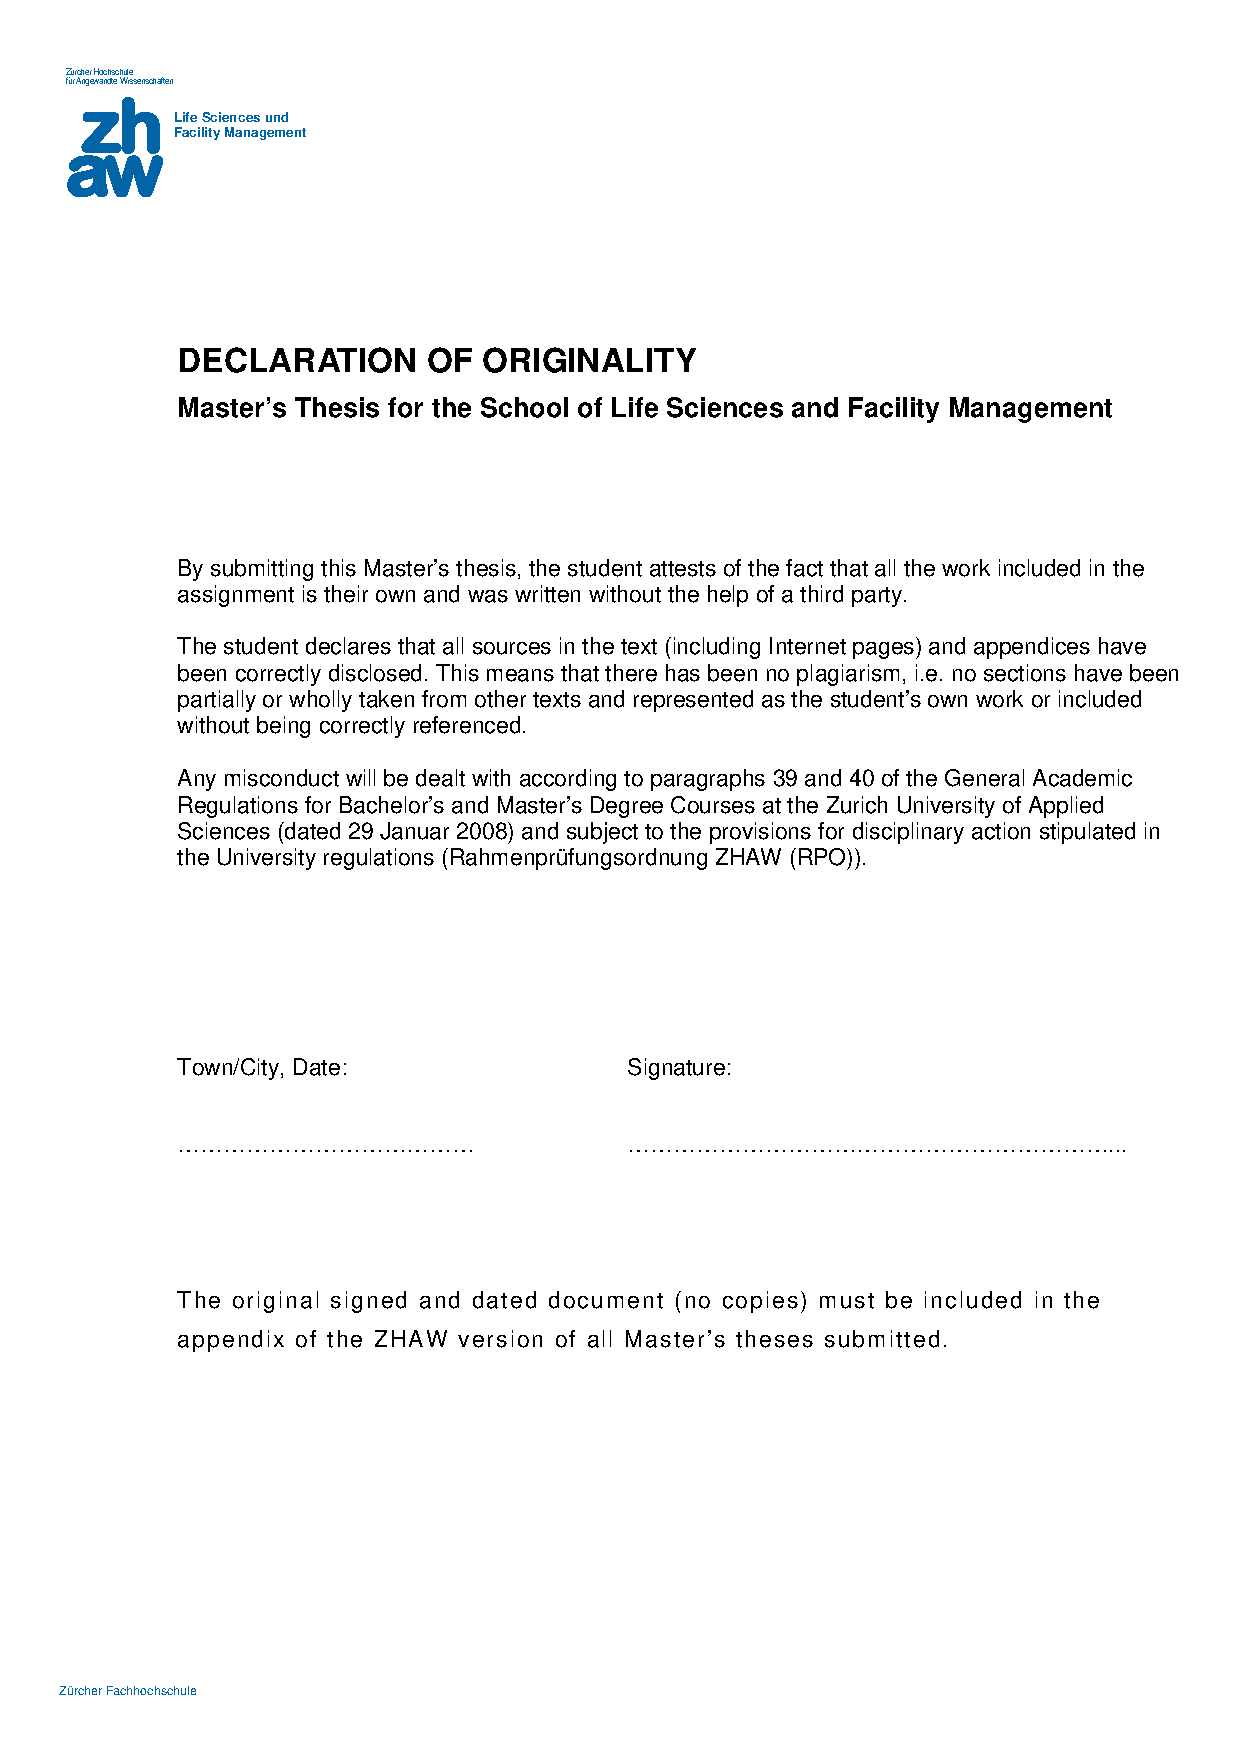
\includepdf[pages=-]{Appendices/plagiatserklaerung-master-eng.pdf}
 


%----------------------------------------------------------------------------------------
% BIBLIOGRAPHY
%----------------------------------------------------------------------------------------
\printbibliography[heading=bibintoc]

%----------------------------------------------------------------------------------------

\end{document}  
